       \documentclass[12pt]{article}

%TODO table des annexes

\usepackage[utf8]{inputenc}
\usepackage[T1]{fontenc}
\usepackage[a4paper,left=2cm,right=2cm,top=2.5cm,bottom=2cm]{geometry}
\usepackage{pdfpages}
\usepackage{hyperref}
\usepackage[titlepage,twoside,fancysections,sectionmark]{polytechnique}
\usepackage[french]{babel}
\usepackage{qrcode}
\usepackage{graphicx}
\usepackage{wrapfig}
\usepackage{tikz}
\usetikzlibrary{matrix}
\usetikzlibrary{arrows,positioning}

\title{Rapport de stage}
\subtitle{Probespoke}
\author{Etienne Bonnafoux}
\date{De juin à août 2018}

\begin{document}
\maketitle
% Page blanche numéroté : II
\newpage
\strut
\newpage
\clearpage

% Avant textes numéroté en chiffres romains à la suite du II précédent
\chapter*{Résumé opérationel}
En Octobre il m'a été proposé de partir trois mois en Thailande afin d'aider l'entreprise du tailleur attitré de l'Ecole Polytechnique à refaire son système informatique. Bien qu'ayant peu d'intéret ni dans le textil ni dans la gestion de système informatique, le challenge m'intérressa.


Je pus y découvrir la gestion d'une très petite entreprise (TPE) dont l'activité se doit d'être internationalisé. Celà demande une gestion particulière des resources et une organisation méticuleuse.


J'ai pu intégrer de nouveaux outils et méthode pour travailler de façon collaborative, avec le moins de risque pour les systèmes critiques de l'entreprise et avec le minimum de perte de continuité.

\vspace{3cm}
\section*{Remerciments}

Je voudrais tout d'abord remercier chaleuresement M. Gerbron pour avoir encadré ce stage. Mes remerciments vont également au Colonel Gaillot pour nous avoir \textit{driver} durant le choix puis le rendu du stage. Je n'oublie pas bien sûr M. Saska Christophe pour m'avoir offert ce stage si intéressant, M.  Perez Torrents Joel pour les nombreuses et fructueuses heures de travaux collectifs passées ensemble, Mme Boonrangsee pour son aide dans les démarches administratives thailandaise et Mme Dang pour nous avoir fait visiter les endroits les plus pittoresques de Bangkok.

\clearpage
\tableofcontents
\clearpage
Ceci est mon intro
\clearpage
\chapter{Description et analyse d'une entreprise atypique: Probespoke}
\section{ProBespoke une entreprise innovante}

\paragraph{}
Probespoke a été fondé en 2012. Il s'agissait tout d'abord de réunir les différentes usines textiles de Bangkok.
Une plateforme informatique commune devais permettre la distribution des commandes venant d'Europe et d'Amérique du Nord.
\paragraph{}
\begin{wrapfigure}[12]{o}{8cm}
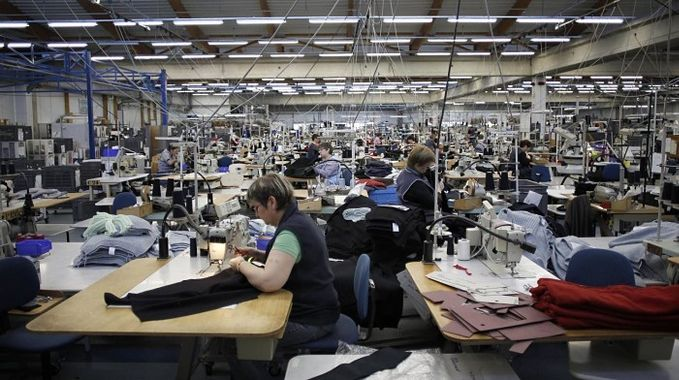
\includegraphics[width=8cm]{image/textile.jpg}
\caption{Une usine quelque part}
\end{wrapfigure}
Mais une différence de point vus à fait éclater le projet. Un des fondateurs, Christophe Saska décida de reprendre le projet sous une forme différente. Il agit comme un trader entre des tailleurs principalement européeen et américain et les usines thailandaises. En effet la fabrication d'une pièce sur mesure est décomposé sur plusieurs poste sur la chaine de fabrication. Une équipe s'occupe que des manches, une autre des poches, et ainsi de suite. Ces équipes ont besoin d'être formées par des maitres tailleurs expérimenté afin de correspondre aux attentes qualités du client. Cette charge de travail est difficile à supporter pour des tailleurs occidentaux peut habitués aux façon de travailler en Thailande. Du côté des ateliers thailandais, cet intermédiare leur permet de ne pas avoir à s'occuper du démarchage des clients. Il s'agit donc d'une opportunité pour tout le monde.

\clearpage
\subsection{Analyse de la stratégie Probespoke}
\paragraph{}
La plus value apportée par Probespoke vient de deux facteurs: la simplification apportée aux tailleurs occidentaux et la différence du coup de main d'oeuvre. Plusieurs zones économiques se partagent le sur-mesure. On peut classer ces zones en deux groupes. Le premier est celui des pays qui ont une forte tradition dans ces domaines à savoir l'Angleterre, la France et l'Italie. Ils se spécialisent dans le sur-mesure haut de gamme à des prix atteignant souvent 1000 euros pour un costume complet. Le deuxième groupe est composé des pays ayant développé plus tardivement une industrie textile dans ce domaine. Il est notamment composé de la Chine, la Thailande, l'Europe de l'Est et le Maghreb. Cette zone produit des costumes de basse et moyenne qualités entre 200 euros et 700 euros. Les équipes sont néanmoins souvent formés par des maitre-tailleurs européens.  Les principaux importateurs sont les États-Unis, l'Europe et plus récemment la classe moyenne asiatique qui s'enrichit.
\paragraph{} Quels sont les aventages (et les incovénients) de s'implenter en Thailande par rapport aux autres pays du même groupe? En Thailande la main d'oeuvre est moins chère qu'au Maghreb et en Europe de l'Est mais plus qu'en Chine. Cependant le dévellopemment du sur-mesure en Chine est plus récent et leur organisation n'est pas encore mature. Ainsi de nombreuses étapes de la confection sont sous-traité ce qui augmente les erreurs de communications. Ainsi de nombreux revendeurs attirées tout d'abord par les prix chinois reviennent ensuite en Thailande. Ce mouvement s'est accélérer cet été, en effet le désaccord commerciale sino-américain pousse de nombreux taileurs américains à quitter la Chine. L'Europe est un marché plus difficile à atteindre; en effet les taxes d'import rendent l'Europe de l'Est et le Maghreb (qui profite d'accord commérciaux) compétitifs devant les prix thailandais. Finalement un atout de la Thailande est son industrie du divertissement. En effet dans de nombreuses entreprises thailandaises il existe un entertaiment officier chargé d'ammener les négociateurs dans des boites de nuits et à d'autres activités illégales pour faliciter la signature des contrats.
%TODO diagramme MIE

\clearpage
%\subsection{Étude stratégique de ProBespoke}
Politiques : stabilité gouvernementale, politique fiscale, protection sociale, commerce extérieur, etc.
Économiques : cycle économique, évolution du PNB, taux d'intérêt, politique monétaire, inflation, chômage, revenu disponible, etc.
Sociologique : démographie, distribution des revenus, mobilité sociale, consumérisme, niveau d'éducation, attitude de loisir et de travail, etc.
Technologiques : dépenses publiques en R&D, investissements privés sur la technologie, nouveaux brevets ou découvertes, vitesse de transfert technologique, taux d'obsolescence, etc.
Écologiques : lois sur la protection de l'environnement, retraitement des déchets, consommation d'énergie, etc.
Légaux : lois sur les monopoles, droit du travail, législation sur la santé, normes de sécurité, etc.

L'entreprise ProBespoke évolue dans un milieu changeant rapidement et sa petite taille ne lui laisse que peu de marge de maneuvre.

Tout d'abord le protectionnisme économique naissant dans les pays occidentaux et surtout aux États-Unies pourait être une menace. Hors à y regarder de plus près les mesures pénalisent surtout ses concurrents directs chinois. Une autre menace politique serait celle d'en changement de régime en Thaïlande qui reste un pays mouvementé.

Ces divers éléments sont résumé dans l'annexe deux, \textit{Matrice SWOT}

%\clearpage
\subsection[Contexte social et écologique]{Une entreprise dans un contexte social et \\écologique}
\paragraph{Impact sur l'Environnement}
\begin{wrapfigure}[12]{o}{8cm}
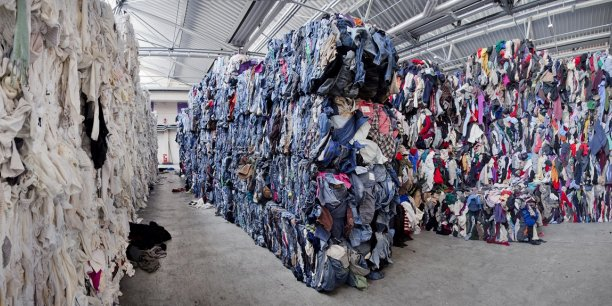
\includegraphics[width=8cm]{image/recyclage.jpg}
\end{wrapfigure}
L'industrie du textile est maintenant la deuxième industrie la plus polluante après la production pétro-chimique\footnote{www.commeuncamion.com/2018/09/02/pourquoi-la-mode-est-devenue-une-des-industries-les-plus-polluantes/}. Pourtant cette question est peu présente dans l'industrie du sur mesure. Il peut néanmoins servir d'argument commercial pour le sur-mesure de luxe qui produit souvent au Portugal. Sinon peux de clients s'intéresse à la provenance de leurs costumes. Une petite étude auprès de mes camarades m’a appris qu'une majorité ne savais pas que leurs costumes venaient de Thaïlande. Quel est son impact par rapport à l'industrie du prêt à porter. En premier lieu, un habit sur mesure sera en général garder plus longtemps qu'une pièce de la \textit{fast fashion}. Cependant les délais de livraison extrêmement cours demandés obligent des trajets aériens intercontinentaux contrairement aux vêtements ordinaires arrivant principalement par voie maritime.
\paragraph{Aspect sociologique}
Les entreprises françaises ont obligation de se renseigner sur leurs fournisseurs, c'est la Responsabilité Sociale des Entreprise (RSE)\footnote{www.e-rse.net/definitions/rse-definition/}. Nous pouvons néanmoins nous demander dans quelle mesure les tailleurs s'intéresse réellement aux conditions de travail des employés du textile en Thaïlande. En effet il est courant d'avoir un atelier \textit{"de démonstration"} et une usine plus effective. Cependant j'ai pu durant mon stage visiter une usine (sans prendre de photo). Les conditions de travail sont correctes avec des locaux climatisés et des postes assis ergonomiques. Ces métiers recrutent autant de femme que d'homme qui sont payés également, ils sont en effet rémunérés à la pièce. D'après notre employeur ce mode de paiement est réclamé par les employés car cela leurs permettrait de prendre des jours chômés quand ils le souhaiteraient.

\clearpage
\section{Mission}

\paragraph{Description}
L'entreprise ProBespoke détenais des solutions technologiques mises en place en 2014.
Cependant une absence de suivi et de maintenance et fortement dégradé le système. L'entreprise possède deux sites vitrines, www.bgc.paris et www. probespoke.com, qui sont statiques et demande donc peu d'entretien.
Probespoke a également mis en place une application disponible sur IOs et Android relié à une plateforme ERP (entreprise resource planing). Cette plateforme est construite avec le logiciel open-source odoo.
 Toutes ces solutions sont sur des serveurs AWS (Amazon Web Service) dont les tarifs obscurs ont mal été compris.
\subsection{Travaux technique}
\paragraph{}
 Ma première mission fut de migrer ces serveurs d'AWS vers les serveurs de l'entreprise OVH et faire ainsi passer les coûts fixes d'informatique de l'entreprise de \$1800 à \$500.
 Pendant cette migration j'ai dû également mettre la dernière version de Odoo, pour passer de Odoo 8 à Odoo 11.
 Lors de cette mise à jour des modules codés il y a quatre ans se sont mis à dysfonctionner, j'ai donc dû en recoder une bonne partie. Finalement j'ai rajouté une fonctionnalité de prise de commande rapide sur l'application et permis sa rediffusion.
 \paragraph{}

 \begin{figure}[!h]
 \centering
 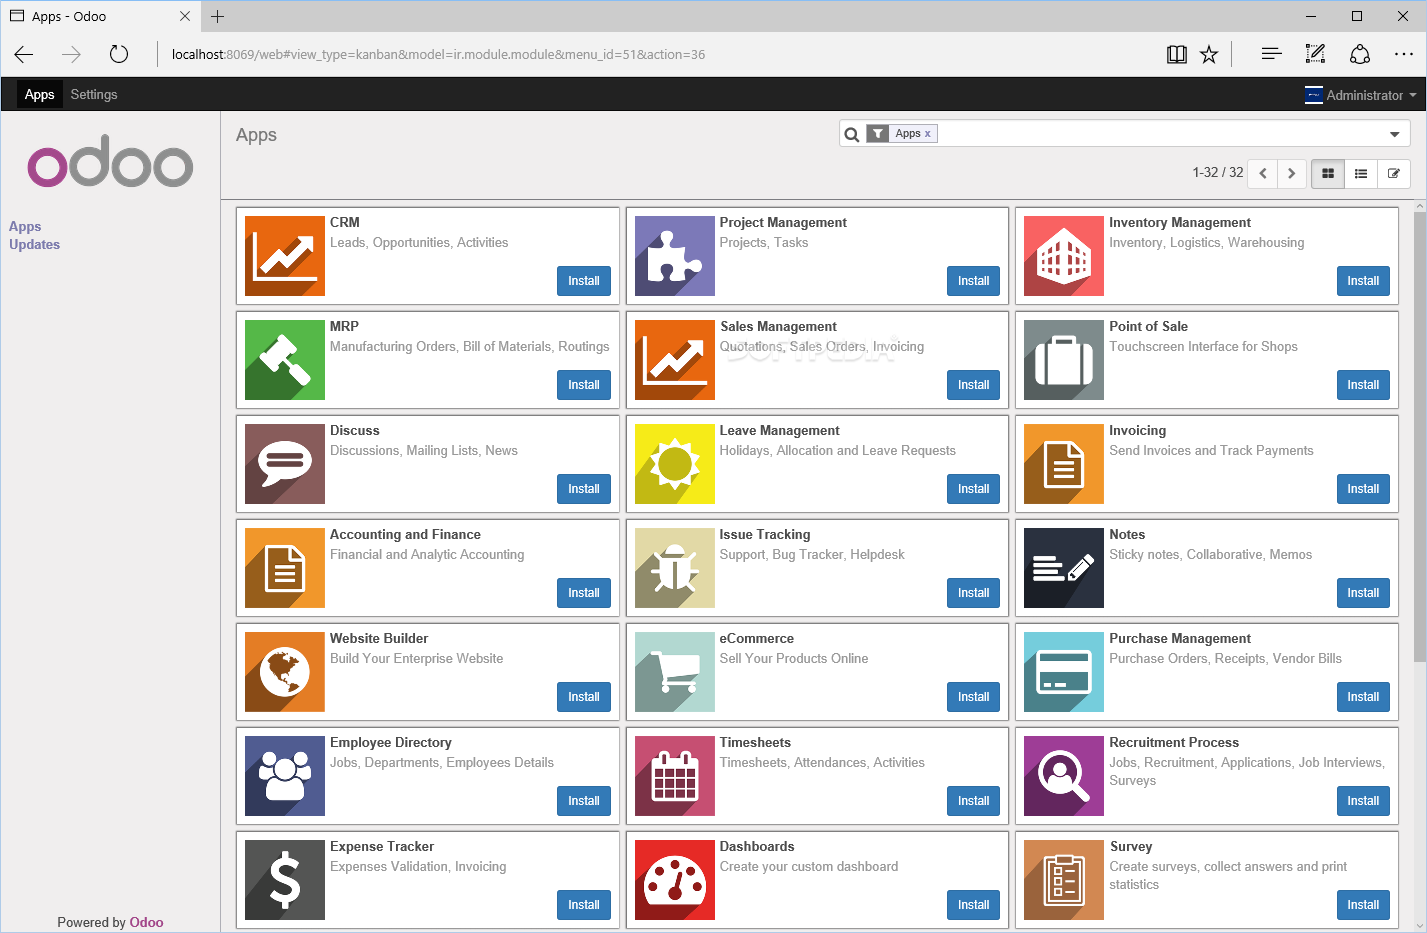
\includegraphics[width=12cm]{image/odoo.png}
 \caption{Différents modules proposés par Odoo}
 \end{figure}

 \subsection{Conseil à l'entreprise}
 \paragraph{}
 Notre employeur n'a pas pour spécialité l'informatique. Ainsi j'ai dû faire des benchmarck pour trouver par exemple la solution d'hébergement de ses serveurs qui sera la moins chers. Je l'ai également mis en garde à propos de certain avancés technologiques qui le pousseront à moyen terme à une réorganisation de ses services. Finalement il m'a également été sollicité pour aider à écrire une demande de devis pour poursuivre la mise en place de son système informatique. Etant pris par son rôle commercial, notre employeur n'a peu de temps pour s'intéresse aux avancés technologiques. De plus ProBespoke n'engage pas d'informaticien à temps plein, ainsi les avancés dans ce domaine sont saccadées. De mon point de vue cela est une erreur étant donné la place prédominante de l'informatique dans cette entreprise.
 \paragraph{}
 \begin{figure}[!h]
 \centering
 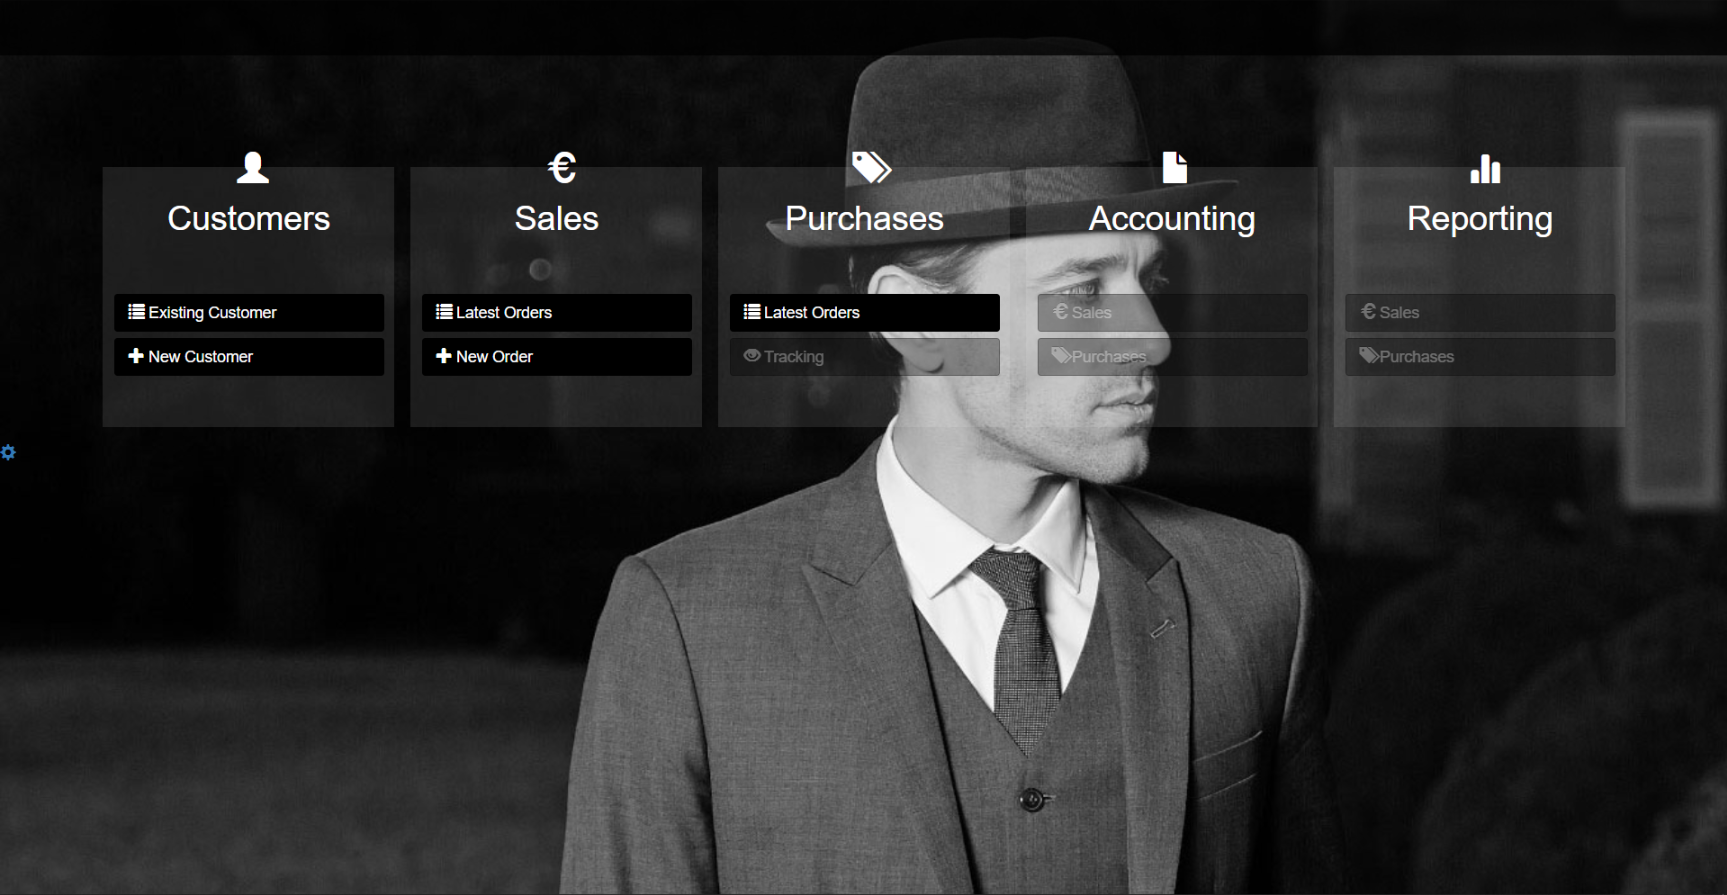
\includegraphics[width=16cm]{image/prise.png}
 \caption{Application de prise de commande}
 \end{figure}

  \subsection{Cadre de travail}
  \paragraph{}
L'entreprise ProBespoke a eu, au cours de son existence, plusieurs prestataires chargés de développer la partie informatique. Ainsi au début une personne nommé Guillaume (je n'ai jamais eu son nom de famille) développa l'application et le logiciel de gestion. Cependant pour une raison que je devine mal un désaccord c'est installé entre lui et M. Saksa le créateur. Puis ProBespoke est passé par une agence pour remettre en place le site internet qui avait besoin de maintenance. Cependant les tarifs étaient prohibitifs pour une petite entreprise comme ProBespoke.
  \paragraph{}
  C'est pourquoi il fut choisi de prendre deux stagiaires ayant des compétences en informatique, ce qui tombait bien car M. Saksa avait pour habitude de vendre des costumes dans des écoles d'ingénieurs. Comment persuader des stagiaires de venir travailler dans son entreprise. Il fut décidé qu'aucun salaire ne serait versé, en revanche le cadre de travail devait être idéal. Ainsi nous eûmes droit à un appartement avec piscine, gym et sauna, quelques repas au restaurant et parfois des soirées au golf. D'un autre côté les horaires était très variables et les journées pouvait être longue et il fallait rester en alerte même le week-end. Cela m'a fait prendre conscience que le salaire est loin d'être la seule variable dans le choix d'un emploie. \begin{figure}[!h]
   \centering
   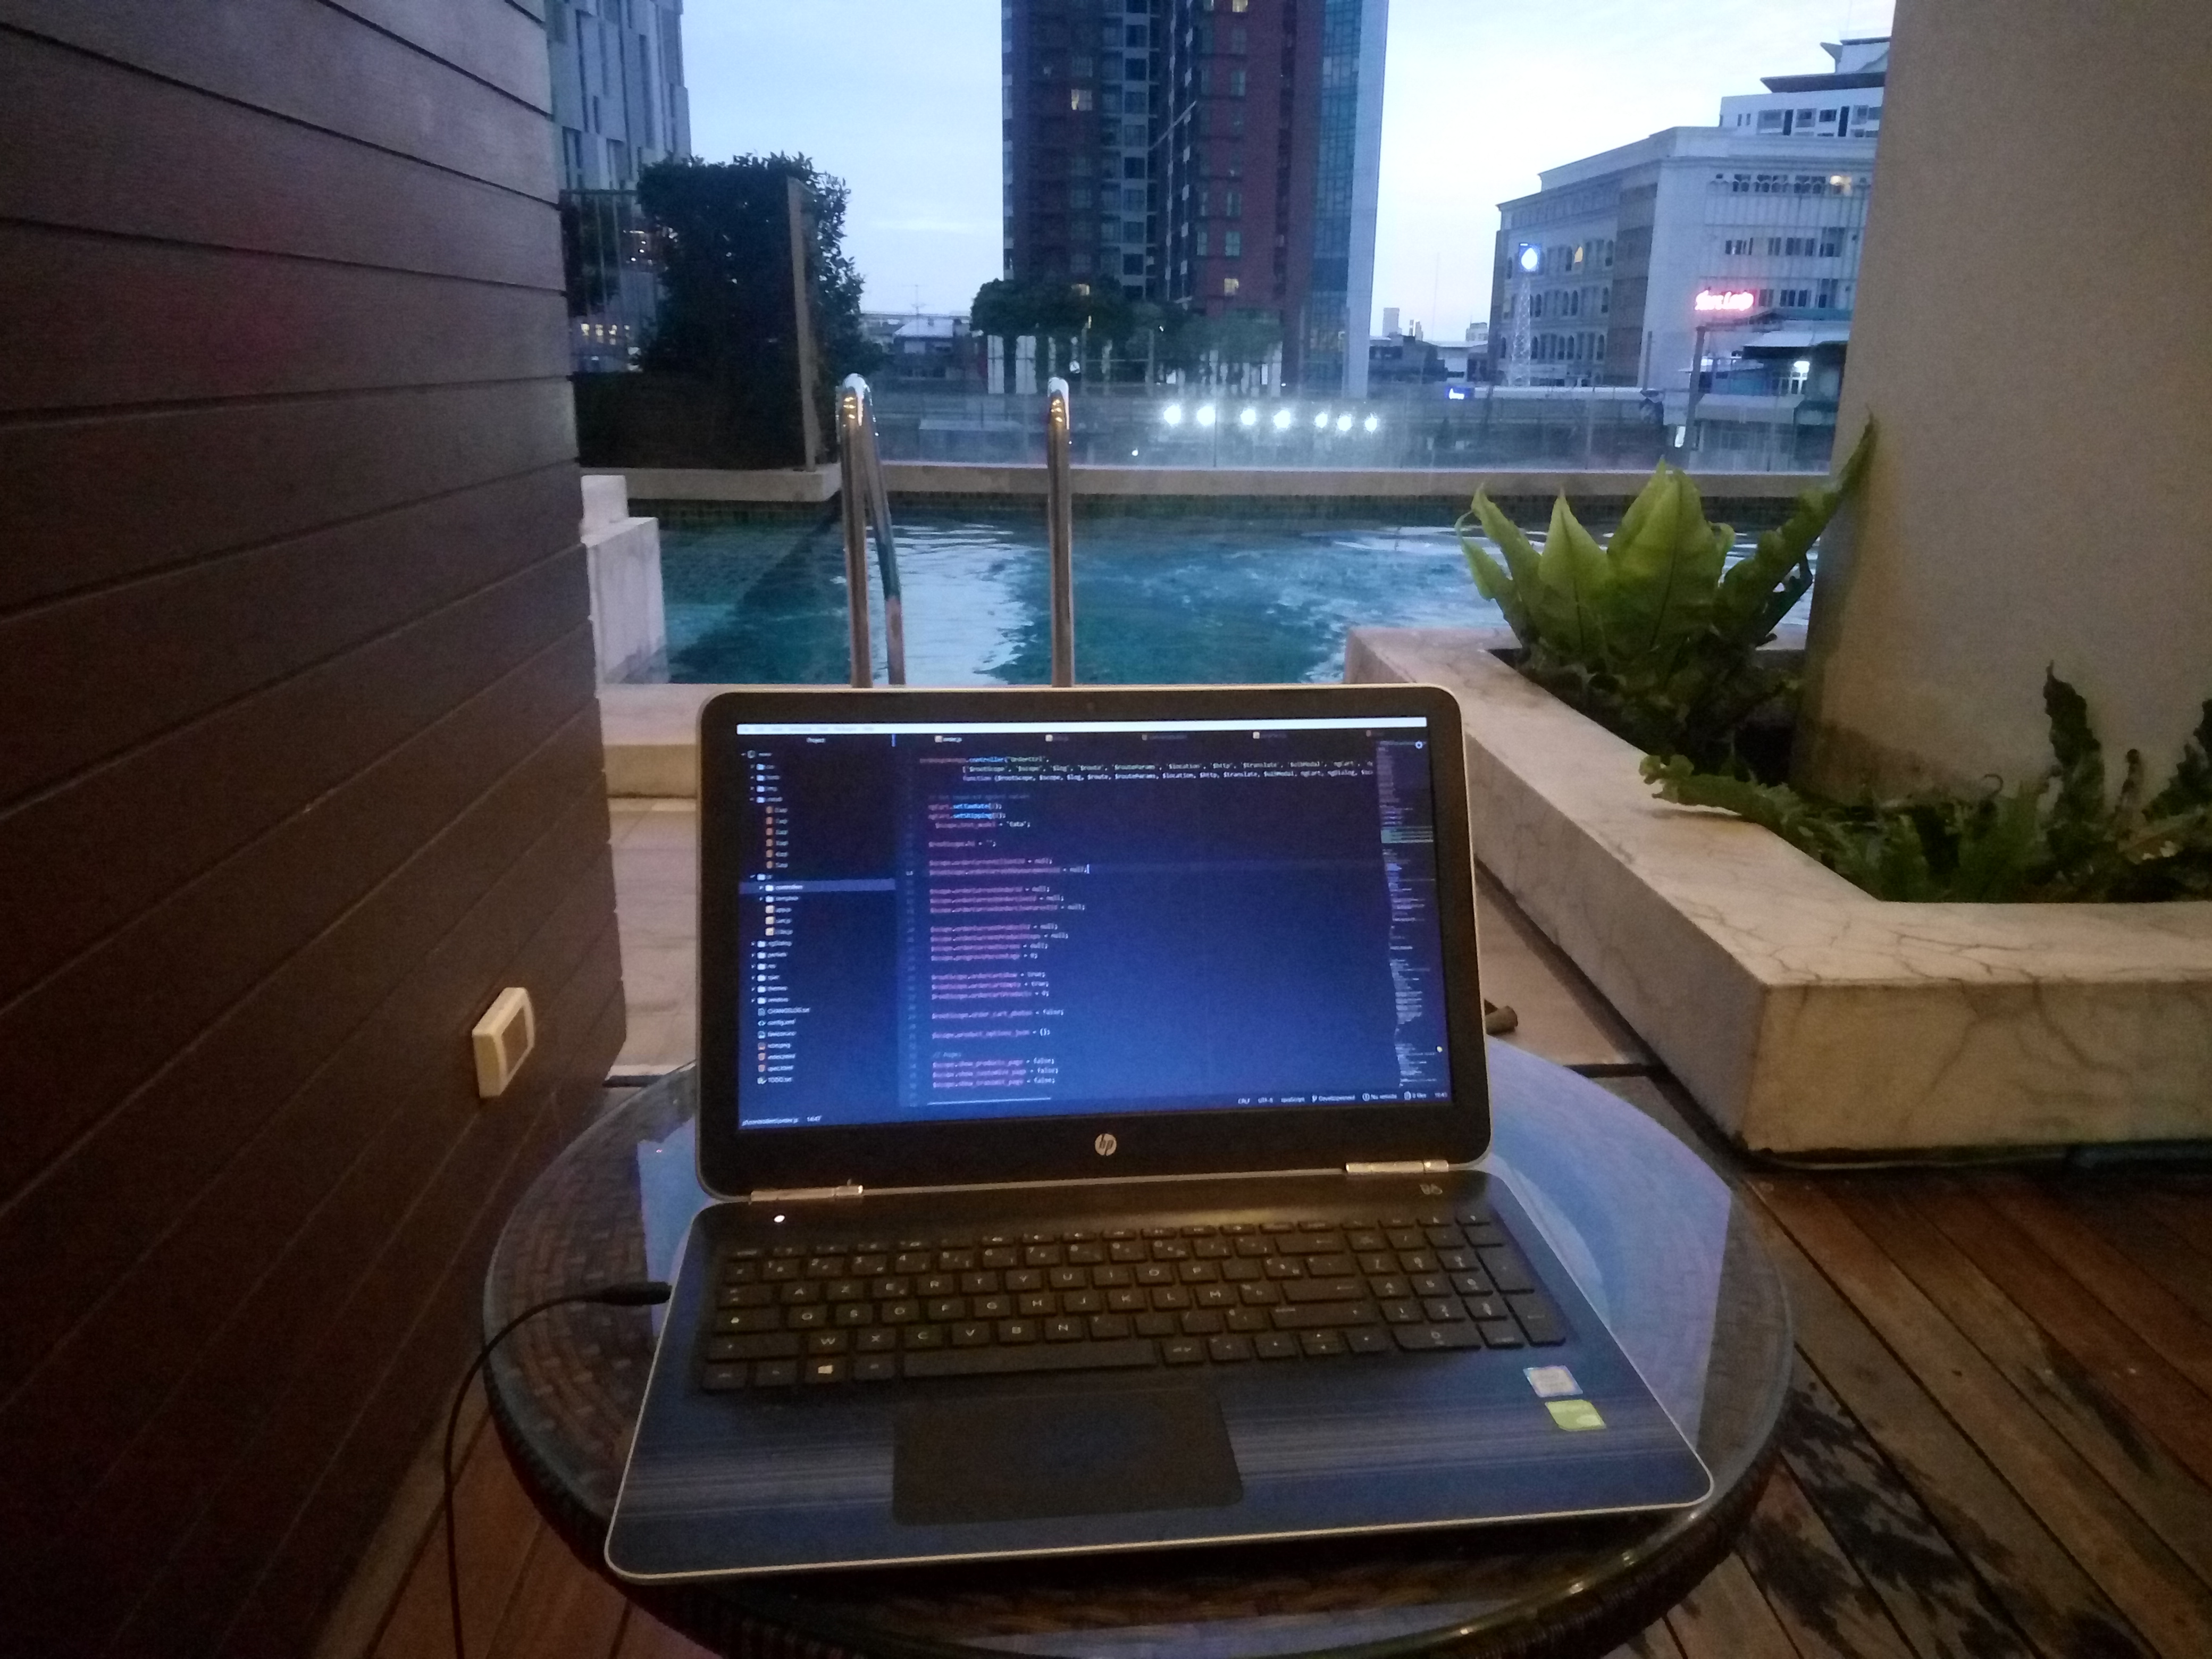
\includegraphics[width=12cm]{image/piscine.jpg}
   \caption{Programmation au bord de la piscine}
   \end{figure}
\paragraph{}
J'aimerais également revenir sur la dispute entre M.Saksa et son précèdent informaticien Guillaume. En effet à cause de cet évènement, ils nous étaient difficile d'avoir un historique de ce qui avait été fait car la personne la mieux placée pour témoigner n'était plus là. Le code était peu documenté, et les explications parfois obscures et incomplète. Nous avons dû une fois écrire un mail au fameux Guillaume ce qui mit fortement mal à l'aise notre patron qui ne voulait pas s'abaisser à lui demander quelque chose. J'en retire également un enseignement. Toujours demander à ses employés de laisser une trace explicative de leurs travaux et toujours essayer de se quitter en bon terme surtout quand cela touche une partie critique de l'entreprise.

\clearpage
\section{Enrichissements personnels}
\subsection{Commentaire sur l'activité professionnel}

\begin{wrapfigure}[24]{o}{8cm}
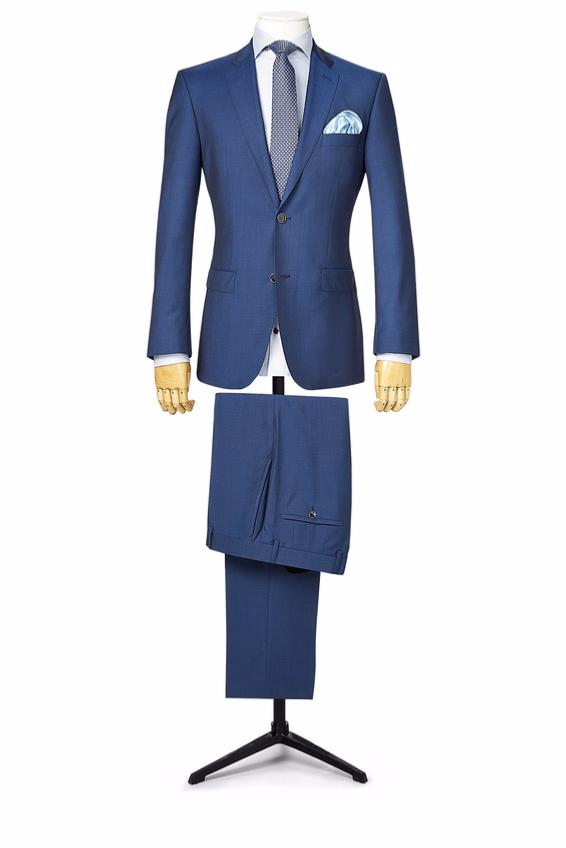
\includegraphics[width=8cm]{image/bleuciel.jpg}
\end{wrapfigure}
\paragraph{Les outils de travail collaboratif}
Ce stage m'a permis de me former à des méthodes de travail efficace et sûr. Tout d'abord j'aimerais parler des outils de travail collaboratif qui ont été mis en œuvre durant ce stage. Le premier et le plus connus est le service de stockage en ligne Google Drive. Lors de notre arrivé, notre tuteur nous a partagé deux dossiers contenant les informations nécessaires pour le stage (mot de passe, code source des applications). Mais ces informations était mal rangée, dédoublé et avait souvent des noms peu explicite (par exemple : "mdp1,password") et cela nous a fait perdre un temps considérable. Je pense donc qu'une classification stricte des ressources et une nomenclature fixée et connue de tous les acteurs sont nécessaire au bon fonctionnement d'une entreprise. J'ai donc utilisé des outils plus professionnels tel Github pour gérer les version du code source des applications et laisser une trace intelligible des modifications apportées à mes potentiels successeurs. Cependant la version privée de Github étant payante, se ne peut pas être une solution à long terme pour ProBespoke.

\paragraph{Une communication efficace}
J'aimerais également mettre le doigt sur un aspect que je pense discriminant dans la conduite d'un projet réussi, la communication. Nous avons vécu durant notre stage deux sortes de périodes. La première était quand notre employeur était en Thaïlande ; nous avions alors l'habitude de travailler seul le matin, puis il nous rejoignait pour discuter des avancés entre 15h et 19h. L'autre période était ses voyages en France. Nous avions alors qu'une heure de discussion chacun au téléphone par jour. La vitesse de progression des différents projets s'en est fortement ressentit. Ainsi une mise au point régulière et efficace est selon moi une aide pour l’avancer d'un projet. Une entreprise souffre rarement d'un surplus de communication, en revanche l'inverse peut se produire. Pour nuancer, il faudrait ajouter que la longueur de l'échange n'est pas forcément proportionnelle à la quantité d'information échangé. En effet souvent nos discussions revenaient sur des points déjà présenté et se perdais en longueur.

\paragraph{Definir son domaine d'activité}
Une autre leçon importante que je retire de ce stage est qu'il faut connaitre sa place. En effet il faut pouvoir annoncer sans modestie ce que l'on est capable de faire, et d'un autre côté ne pas se montrer trop téméraire en annonçant des choses hors de nos disponibilités. Notre employeur qui prend des mesures dans différentes écoles, d'ingénieur et de commerce, nous a fait remarquer que la plus grande faiblesse des X est qu'ils ne savent pas se vendre. En effet peu d'entre nous comprennent à quel point leurs compétences peuvent être rare et recherchée ; ils ne les mettent donc pas en avant. D'un autre côté, il faut connaitre ces limites. J'ai notamment dû convaincre notre employeur de nous laisser quelque jour de recherche avant de se lancer dans une tâche critique, la migration d'un serveur. Effectivement il n'évalué pas bien, à mon avis, le risque des différentes opérations et la complexité qu'il y aurait à réparer la situation.

\paragraph{Définir les besoins du clients}
Finalement une autre composante critique dans une opération est de bien définir un cahier des charges. Cela peut être d'autant plus difficile que le client maitrise peu le langage technique voir qu'il ne connaisse même pas la possibilité de certaines options. Il faut donc construire avec lui une définition précise de son besoin. Plusieurs outils existent notamment les diagrammes de séquences\footnote{fr.wikipedia.org/wiki/Diagramme\_de\_sequence}  ou bien l'\textit{Unified Modeling Language} \footnote{openclassrooms.com/fr/courses/2035826-debutez-lanalyse-logicielle-avec-uml/2035851-uml-c-est-quoi}. Durant mon stage peu d'entre eux ont été mis en œuvre. Heureusement des rencontres ponctuelles avec notre employeur permettent de rectifier le cap régulièrement, mais sans cela le projet aurait bien pu ne pas aboutir.

\clearpage
\subsection{Vision sur mon projet professionnel}
%TODO illustration
\paragraph{}
Pendant ce stage il m'a également été demandé de réfléchir sur mon orientation et mon avenir professionnel. J'ai particulièrement apprécier durant se stage les réflexions qui m'a été demandé de faire. J'ai également compris que la prise de responsabilité n'était pas quelque chose qui pourrait me gêner. J'aimerais donc m'aurienter vers des métiers présentant des défis intellectuels. Il me serait ainsi difficile de faire un métier où les solutions sont toutes trouvées et il ne faudrait qu'appliquer une méthode.

\paragraph{}
Je voudrais être également créateur. C'est pourquoi je pense m'orienter vers les métiers de la recherche. Le domaine informatique est intéressant mais ne me correspond pas tout à fait. Je pense plutôt faire des mathématiques appliquées ou pures. C'est pourquoi j'ai choisi le programme d'appronfondissement en mathématique en troisième année. je voudrais après avoir un master en mathématique, faire une thèse.

\paragraph{}
Le fait que se stage fût dans un pays étrangé m'a également plu. J'aime beaucoup confronter ma vision du monde et ma façon de travailler à la réalité d'un autre pays. Ainsi j'espère pouvoir faire une carrière tournée vers l'international.

\clearpage
\chapter*{Conclusion}
Une petite conclusion qui est très sympa


% Après textes numéroté en chiffres romains à partir de
\clearpage
\appendix
%\section*{Annexes}
\renewcommand{\contentsname}{Table des annexes}
%TODO table des annexes
%\tableofcontents
\clearpage
%\addcontentsline{toc}{subsection}{Glossaire}
\section{Glossaire}

%TODO a faire mieux
\paragraph{ERP : }
\begin{wrapfigure}[4]{o}{4cm}
\qrcode[height=1in]{https://en.wikipedia.org/wiki/Enterprise_resource_planning}
\end{wrapfigure}
\paragraph{}

\textbf{E}nterprise \textbf{R}esource \textbf{P}lanning  en anglais. Outil informatique permettant de mettre en lien différente partie d'une même entreprise. Cet outil doit assurer l'intégrité des ressources ainsi qu'il doit premettre de faire des audits.

\paragraph{Odoo : }
\begin{wrapfigure}[5]{i}{4cm}
\qrcode[height=1in]{https://www.odoo.com/fr_FR/}
\end{wrapfigure}
\paragraph{}
Odoo est un logiciel de gestion d'entreprise dont la première version est sortie en 2004. Il comprend plusieurs modules dont la gestion des ventes, des ressources humaines ou de la comptabilité. Si ça version basique est gratuite il existe une version payante incluant un support.

\paragraph{UML : }
\begin{wrapfigure}[5]{o}{4cm}
\qrcode[height=1in]{https://en.wikipedia.org/wiki/Unified_Modeling_Language}
\end{wrapfigure}
\paragraph{}
\textbf{U}nified \textbf{M}odeling \textbf{L}anguage en anglaise. Language et suite de diagramme permettant de définir un cahier des charges dans le domaine informatique. L'analyse se fait d'abord du point de vue du client puis déscend au différentes solutions techniques envisagées et au flux d'information.

\clearpage
%\addcontentsline{toc}{subsection}{Matrice SWOT}
\section{Matrice SWOT}
\newcommand{\texta}{Helpful \tiny (to achieve the objective)\par}
\newcommand{\textb}{Harmful \tiny (to achieve the objective)\par}
\newcommand{\textcn}{Internal origin \tiny (product\slash company attributes)\par}
\newcommand{\textdn}{External origin \tiny (environment\slash market attributes)\par}
\newcommand{\nodestrengths}{Strengths\\\begin{itemize}
  \item Application de prise de mesure
  \item Gestion informatisé des commandes
\end{itemize}}
\newcommand{\nodeweakness}{Weakness\\\begin{itemize}
  \item Barière douanière
  \item Mauvaise image de l'industrie textile en Asie
\end{itemize}}
\newcommand{\nodeopportunities}{Opportunities\\\begin{itemize}
  \item Guerre commercial USA/Chine
  \item Emergence de la classe moyenne asiatique
\end{itemize}}
\newcommand{\nodethreats}{Threats\\\begin{itemize}
  \item Instabilité politique thailandaise
\end{itemize}}
\begin{tikzpicture}[
    any/.style={draw,minimum width=8cm,minimum height=8cm,
                 text width=5cm,align=left,outer sep=0pt},
    header/.style={any,minimum height=1cm,fill=black!10},
    leftcol/.style={header,rotate=90}
]

\matrix (SWOT) [matrix of nodes,nodes={any,anchor=center},
                column sep=-\pgflinewidth,
                row sep=-\pgflinewidth,
                row 1/.style={nodes=header},
                column 1/.style={nodes=leftcol},
                inner sep=0pt]
{
          & {\texta} & {\textb} \\
{\textcn} & {\nodestrengths} & {\nodeweakness} \\
{\textdn} & {\nodeopportunities} & {\nodethreats} \\
};
\end{tikzpicture}

\clearpage
%\addcontentsline{toc}{subsection}{Chiffre du textile}
%\section{Chiffre du textile}
%quelques chiffres sur le textile
Asie 80\% des exportations mondiales
500 milliard de dollars



\end{document}
